\section{Schéma de structure}

\begin{figure}[h]
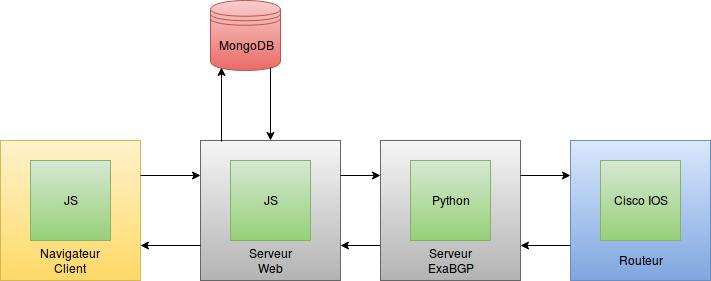
\includegraphics[scale = 0.75]{img/structure.png}
\caption{Schéma de structure}
\end{figure}


\subsection{Structure de la base de donnée}

\begin{center}
\begin{figure}[h]
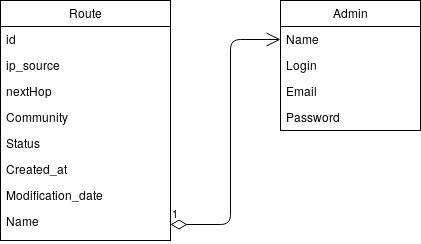
\includegraphics[scale=0.5]{img/table_mongoDB}
\caption{Uml de la base de donnée}
\end{figure}
\end{center}

La table "Route" permettra de stocker toutes les routes annoncées avec plusieurs champs spécifique:
\begin{itemize}
\item id: Une clé unique représenter par un entier positif.
\item Ip source: une adresse ip sous forme ipv4/ipv6, c'est-à-dire pour ipv4 sous la forme de quatre nombres entiers séparés par des points allant de 0.0.0.0 à 255.255.255.255. pour ipv6 8 groupes écrit en héxadécimale séparés par deux-points.
\item NextHop: une adresse ip comme ip source.
\item Community: Un tag décrivant la communauté du routeur une chaîne de caractère.
\item Status: Une chaîne de caractère qui est soit "Activate" ou "Desactivate".
\item Created at: la date de création de la route sous format <YYYY-mm-ddTHH:MM:ss> Y:année m:mois d:jour h:heure M:minute s:seconde.
\item Modification date: la date de la dernière modification sur cette route, peut être vide.
\item Name: le nom de l'administrateur qui la modifier ou ajouter représenter par une chaîne de caractère.
\end{itemize}

La table Admin permettra de stocker tout les administrateurs avec les champs suivants:
\begin{itemize}
\item Name: nom de l'administrateur représenter par une chaine de caractere.
\item Login: pseudonyme de l'administrateur représenter par une chaine de caractère.
\item Email:  une adresse mail valide de l'administrateur.
\item Password: un mot de passe.
\end{itemize}